\title{\textbf{\Huge Book-taste clustering in goodreads communities}}

\author{{\Large Akanksha Tiwari (A0123476E)} \\
    {\Large Antoine Francois Pascal Creux (A0123427M)}\\
    {\Large Ashish Dandekar (A0123873A)} \\\\
    National University of Singapore,\\
    Singapore
}
\date{\today}

\documentclass[11pt]{article}
\usepackage[margin=1in]{geometry}
\usepackage[english]{babel}
% \usepackage{listingstyle}
\usepackage{graphicx}
\usepackage{caption}
\usepackage{subcaption}
% \usepackage{coz}
\usepackage{url}
\usepackage{array}
\usepackage{multirow}
\usepackage{soul}
\usepackage{amssymb}
\usepackage{hyperref}
% \usepackage[autolanguage]{numprint}

\begin{document}
\maketitle

\section{Detailed Problem Description}
Goodreads is a website launched in early 2007, which lets ``people find and share the books they like and improve the process of reading and learning throughout the world.'' It is the world's largest site for readers and book recommendations with a user base of about 30 million members along with 34 million reviews from 900 million books as recorded in 2015 \cite{goodreads:aboutus}.\\\\
Goodreads provides a multitude of features to its users. It goes beyond the traditional rating and reviewing of books by allowing users to make friends and join and form reading groups based on their literary tastes.
Users can not only see what their friends have read, but they can also meet new people with similar reading interests. They can make recommendations to friends, follow authors, track the books they are currently reading, have read and want to read.
In addition, goodreads provides personalized recommendations to book readers by analyzing the user data.\\\\
Our project aims to detect and study goodreads communities based on the book ratings given by users.Through this analysis we seek to understand whether the communities detected based on similar book tastes are alike to the friends communities formed by users themselves on goodreads and the extent to which these user communities on goodreads exhibit homophily.
\subsection{Assumptions}
% zero rating

The users who have not provided any ratings for the books that they have read are considered as invalid users and we have eliminated them from our data set. This is because just having read the book does not indicate that the user has liked the book. We also need the rating he has given to the book to know whether he/she likes(high rating) or dislikes (low rating) the book he has read.\\\\
However, as of now we have considered users who have given rating for at least a single book as valid users. The data set right now stores a 0 rating if a user has read the book but has not provided a rating for it. We are still working on how to resolve this. One possible way could be to remove this edge between the user and the book. This again could be debatable as by removing this edge we are losing the information that there is a relation between this user and book.\\\\
The users with private profiles whose data we could not scrape because their reading information is just visible to their friends are also considered as invalid users. So, we have not included them in our data set.\\\\
We are assuming that the data we get from scraping is unbiased. That is, we assume that the group ({\it Goodreads Authors/Users}) whose members, members' friends and their books read that we have scraped is representative of readers from various genres. Indeed, this group is very large and popular and is used to share book experiences across different genres.

\subsection{Objectives}

\begin{itemize}
\item[\checkmark] Gather relevant data (as mentioned in Section \ref{sec:data_acquisition}) from goodreads
\item[\checkmark] Survey various algorithms for community detection on the graphs generated from the data
\item[\checkmark] Analyze and interpret the results of applying these algorithms on the data 
\item[\checkmark] Analyze the extent to which the user groups on goodreads exhibit homophily
\item Study the effect of recommendations and users' friend on his/her choice of books (If time permits)
\end{itemize}

\subsection{Contribution}
As of the literature survey done up to now, there has not been a study on the detection of communities of readers with similar reading interests on goodreads dataset.
This work will aim to identify such communities using algorithms for community detection such as Girvan-Newman algorithm and compare the communities detected with the already formed groups on goodreads and analyze how different or similar they are.
This would give us insights into whether the friendship and groups formed on goodreads are based on reading interests or there are other factors that come into play. It can be especially useful to authors in identifying the right target audience for their work. \\\\
% Are you sure you want to write this?
% In addition, if we get time, we can also look at how the recommendations and friendships in the goodreads' user network affect the choice of books. This information can be used by goodreads themselves to improve their recommendation engine.

\section{Related Work}
\label{sec:related_work}
Our focus is on studying whether the existing groups on goodreads exhibit homophily based on the communities we detect using the user graph generated from the book ratings given by users.Based on the sample we have, the graph is very dense.
With less than 8000 user nodes, we have more than 16 million edges, and thus the density reaches 50 \%.
% Dont really understand the next sentence
Community detection is a widely discussed topic in the social networking literature\footnote{Social networks are generally sparse networks. When the networks are dense, the community detection does not seem to be a wise option. The dense networks possess large number of inter-community edges which yield poor partitioning. For dense networks, discrete data analysis techniques are used.}\cite{clauset}.
% http://onlinelibrary.wiley.com/doi/10.1002/wics.1319/pdf
% Advanced Review Community detection in large-scale networks: a survey and empirical evaluation
Finally, we also studied different community detection algorithms. Tens of them, if not hundreds exist in the social network analysis field. We do not aim at creating, customizing or optimizing our own algorithm. Given the size of our basic user graph, we opt to look for community detection algorithms in large-scale networks. Such algorithms have arisen in the last few years, as specified in \cite{survey}.

Initially, we decided to use the Girvan-Newman algorithm as it is one of the most popular community detection algorithms\cite{newman}. This algorithm uses the ``edge betweenness'' of an edge as the number of shortest paths between pairs of nodes that run along it. Edges with high betweeness are very likely to be the connection between communities.
Thus, removing the edges in the decreasing order of betweenness should reveal the associated dendrogram, and thus the communities. However, this computation takes $O(ne)$ running time, and therefore is too long for our graph.\\

Also, \textit{G-N} can be limiting as every node has to be placed in one unique community.
In order to apply this algorithm, since we are dealing with a bipartite graph, we can try to find complete bipartite subgraphs.
For instance, we can split the users and the books into two distinct sets respectively, such as $users0$ and $books0$, and $users1$ and $books1$ are linked, but no edge connect $users0$ and $books1$, or $users1$ and $books0$.
However, based on our graph density which is pretty high, we cannot apply this algorithm: we could end up getting a unique complete clique.
% However, we could filter the edges.
% For instance, keeping only the edges with a rating of 5.
Filtering the edges is one option we have considered in this project.\\

The Louvain\cite{louvain} method for community detection which has come up in the last few years, is a graph partitioning technique that provides an accurate and computationally efficient approach to detect communities in networks consisting of millions of nodes. We will explore this method in the current study.
% label-propagation
% fastgreedy - clauset moore

% More about commubnity detection
% Overlapping
% Group based, member based
% What algos do we choose and why?
% Maybe wait for results



\section{Data Acquisition}
\label{sec:data_acquisition}
Goodread provides well documented and publicly accessible API to query various features supported by the website. All we need is a developer key, which one gets after signing up on goodreads, and an OAuth access to use numerous APIs. The data of the users on a website, being the concern of privacy, is not readily available by means of goodread APIs. Aside from this a goodread user has liberty to keep his/her profile private making it accessible only to the friends on goodreads. Given the large user-base of goodreads, we hope to get sizable dataset to run our analysis.\\\\
Although the data scraping is laborious and time consuming, its is vital in our study. For a fair study, the data must be unbiased. The method which we use to gather the data may add some bias to it. So selection of scraping method is critical to data acquisition. There are two ways one can collect the data:
\begin{description}
\item[Retrieve User IDs from a group]
Goodreads hosts various reading groups catered to various genres and reading interests. User can become member of such groups or can initiate a group. In a group reading activities are supported wherein members can schedule the book readings so that they can share their opinions and conduct a healthy conversation. {\it Goodreads Authors/Readers} is one of the major groups on goodreads.  According to goodreads, this group is dedicated to connecting readers with goodreads authors. It is divided by genres, and includes folders for writing resources, book websites, videos/trailers, and blogs. A {\it toy dataset} scraped from the group shows the absence of bias in the data.\\
Goodreads provides an API to get the list of users given the ID of the group. One can get the ID of the group from the URL of the corresponding group on goodreads.
\item[Retrieve User IDs from reviews of books]
The list of various books genres is available at \cite{goodreads:genres}. One can select top rated books from the highly reviewed genres. So this collection of ``best-selling'' books forms a base set for the books. So we can get the list of users who have read these books. But goodreads fails to support an API which retrieves reviews for a particular book given its ID. Despite this, a meticulous analysis of \textit{Javascript} calls, the webpage makes to show the reviews of a book to the user, reveals a bacdoor API \textit{book/reviews/}. We can retrieve user related information User ID and the rating by parsing the response to the \textit{Javascript} callback using regular expression.

\end{description}
The list of User IDs thus scraped serve as a base user set. We later collect {\it 1-neighbourhood} of this set of users, namely friends of them and the books read by these friends, to get a substantial dataset.\\
We are using the first strategy to scrape the data off the goodreads. Plus the data related to the friends assures the sizable amount for the analysis.

\subsection{Statistics}

\begin{figure}[ht]
        \centering
        \begin{subfigure}[b]{0.5\textwidth}
                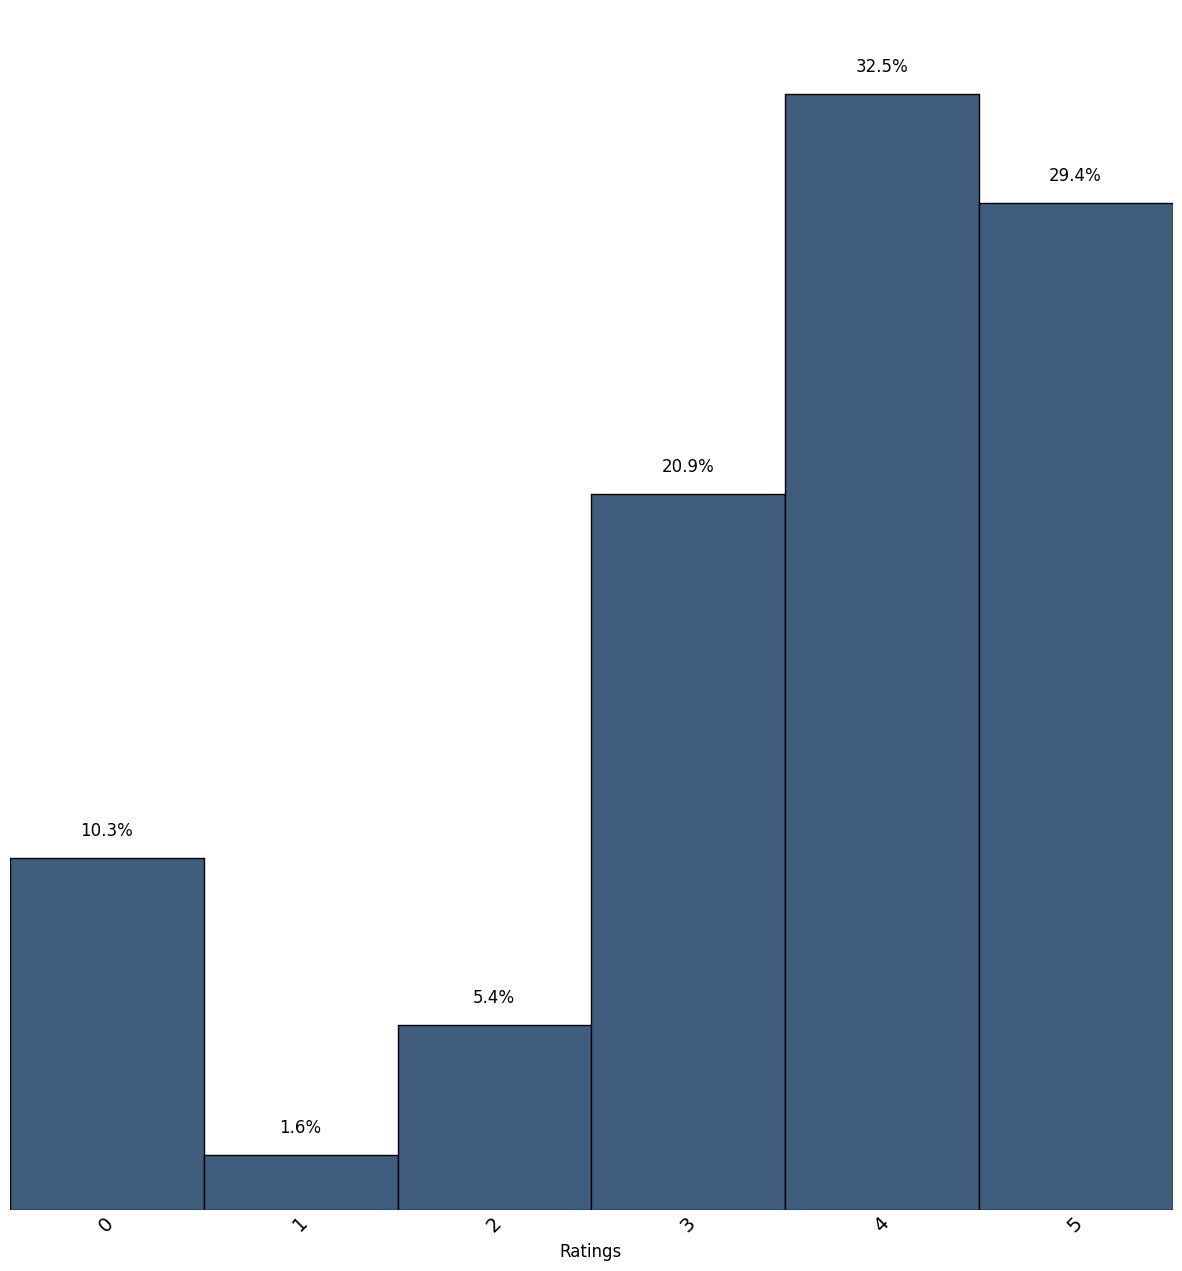
\includegraphics[width=\textwidth]{images/all_ratings}
        \end{subfigure}%
        \caption{Distribution of reviews}
        \label{fig:all_reviews}
\end{figure}


An overview of the goodreads data we have scraped is vital as it helps us understand and grasp insight of the data we are munging.
As it is explained in Section~\ref{sec:data_acquisition}, we have extracted our data in two steps:
\begin{itemize}
\item Members of the Goodreads Authors/Users
\item Friends of the Goodreads Authors/Users members
\end{itemize}

As we can see in Table~\ref{table:crawl_stat}, by getting only the first degree connection of approximately twenty thousand members of {\it Goodreads Authors/Users} group, we have close to 15 million reviews, 1714613 books and 86000 users to analyze. Besides, as we can see in Figure~\ref{fig:all_reviews}, 10\% of reviews were given a rating of 0, which means a reader has not rated the given book.


\begin{table}[ht]
\begin{center}
\begin{tabular}{lcccc}
\hline
                           &  Goodreads Authors/Users    &   Friends                &   All        \\ \hline
\#Ratings                  &  567461                     &   13832047               &   14399503  \\ \hline
\#Users                    &  17583                      &   95503                  &   113086     \\ \hline
\#Public Profiles          &  7816                       &   78723                  &   86538     \\ \hline
\#Private Profiles         &  2564                       &   5314                   &   7878      \\ \hline
\#Profiles w/o any reviews &  7203                       &   11559                  &   18762      \\ \hline
\#Books rated              &  171653                     &   11559                  &   1714613      \\ \hline
\end{tabular}
\end{center}
\caption{Goodreads Authors/Users Statistics}
\label{table:crawl_stat}
\end{table}
% Problem with private profiles. Need data from 100 to 350 for 1st degree connection
% But akanksha has already uploaded the 100 to 350 data

Let's observe a few things in the base dataset.
Users have read an average of $166$ books, whereas a book has been read by approximately $8$ people.
Please refer to Figure~\ref{fig:readers_book_read} to see the detailed user statistics.
As expected, a large portion of the readers which has read less than 50 books.
Figure~\ref{fig:books_books_read} shows the stats for the books.
$54.2\%$ books in the dataset are read/reviewed by a single user.
Only $10$\% of the books have been read by more than $10$ readers.
We recognize the same pattern in music, movies or consuming goods: only a fraction of them has been listened/watched/bought by a significant amount of people.
% Next sentence?
% This stark contrast separate the books which are popular from the ones which are not much popular.
Users have given an average rating of $3.52$ to the books while books have an average of $3.23$.
This difference, even tiny, strengthens the correlation that a well rated book is more likely to be read.

% print c.user_average_book()
% print c.book_average_user()
% print c.user_average_rating()
% print c.book_average_rating()

% 166.39514433
% 8.38730595677
% 3.524460734
% 3.22690806765

\begin{figure}[ht]
        \centering
        \begin{subfigure}[b]{0.5\textwidth}
                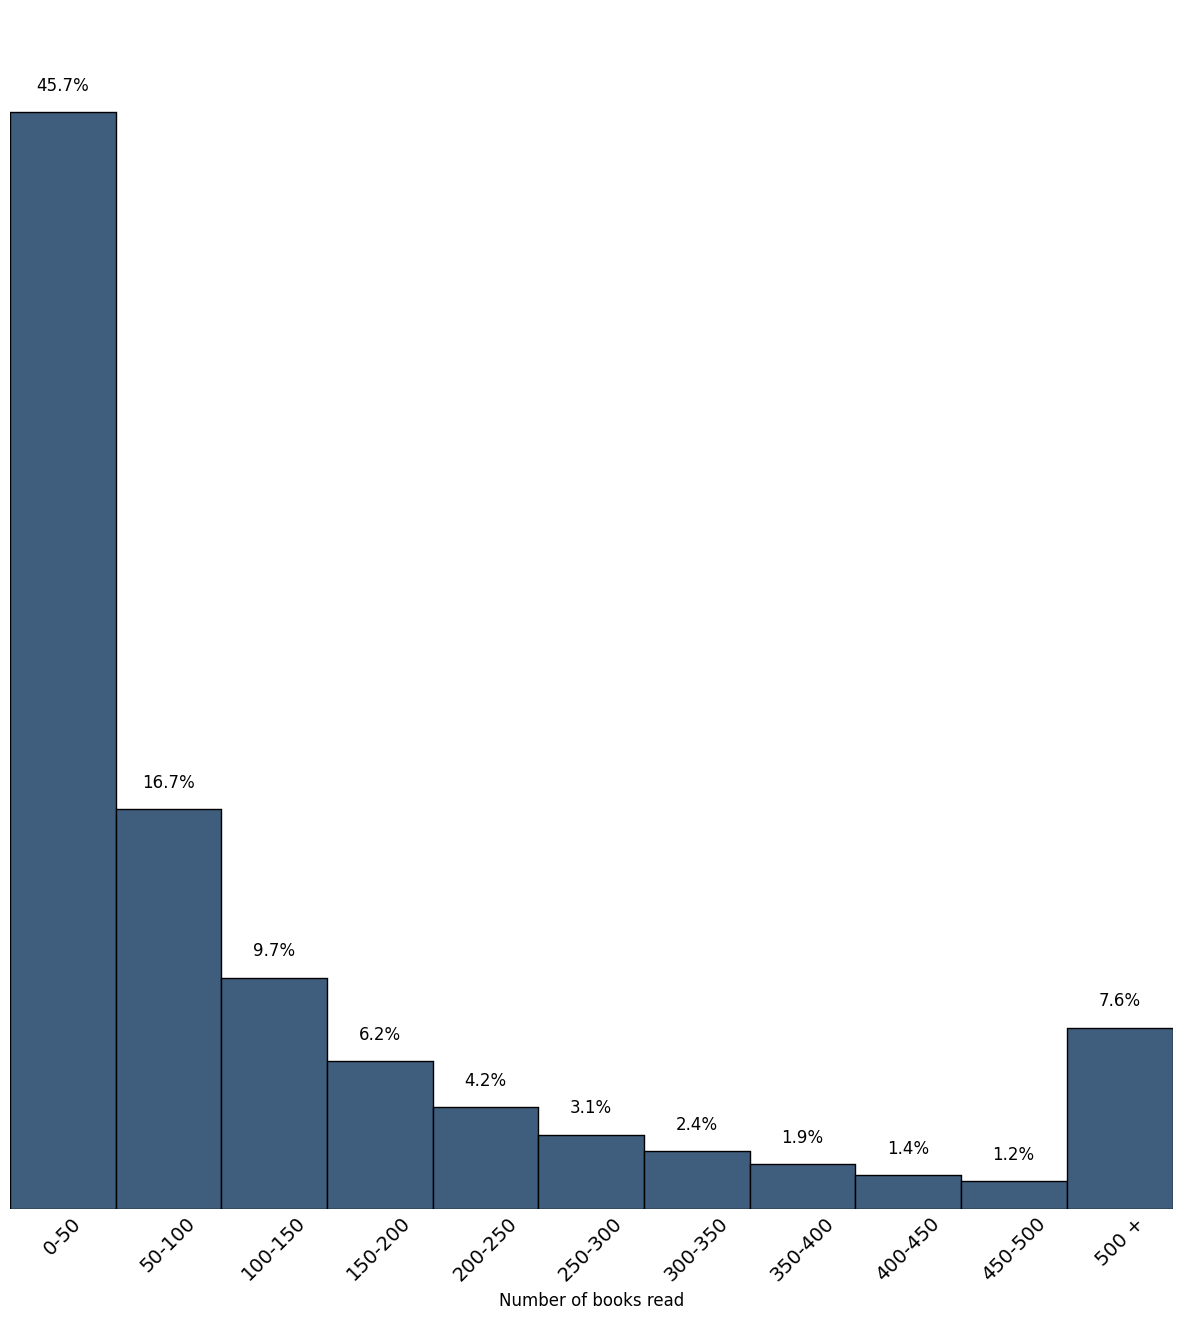
\includegraphics[width=\textwidth]{images/users}
                \caption{Distribution of readers}
                \label{fig:readers_book_read}
        \end{subfigure}%
        ~ %add desired spacing between images, e. g. ~, \quad, \qquad, \hfill etc.
          %(or a blank line to force the subfigure onto a new line)
        \begin{subfigure}[b]{0.5\textwidth}
                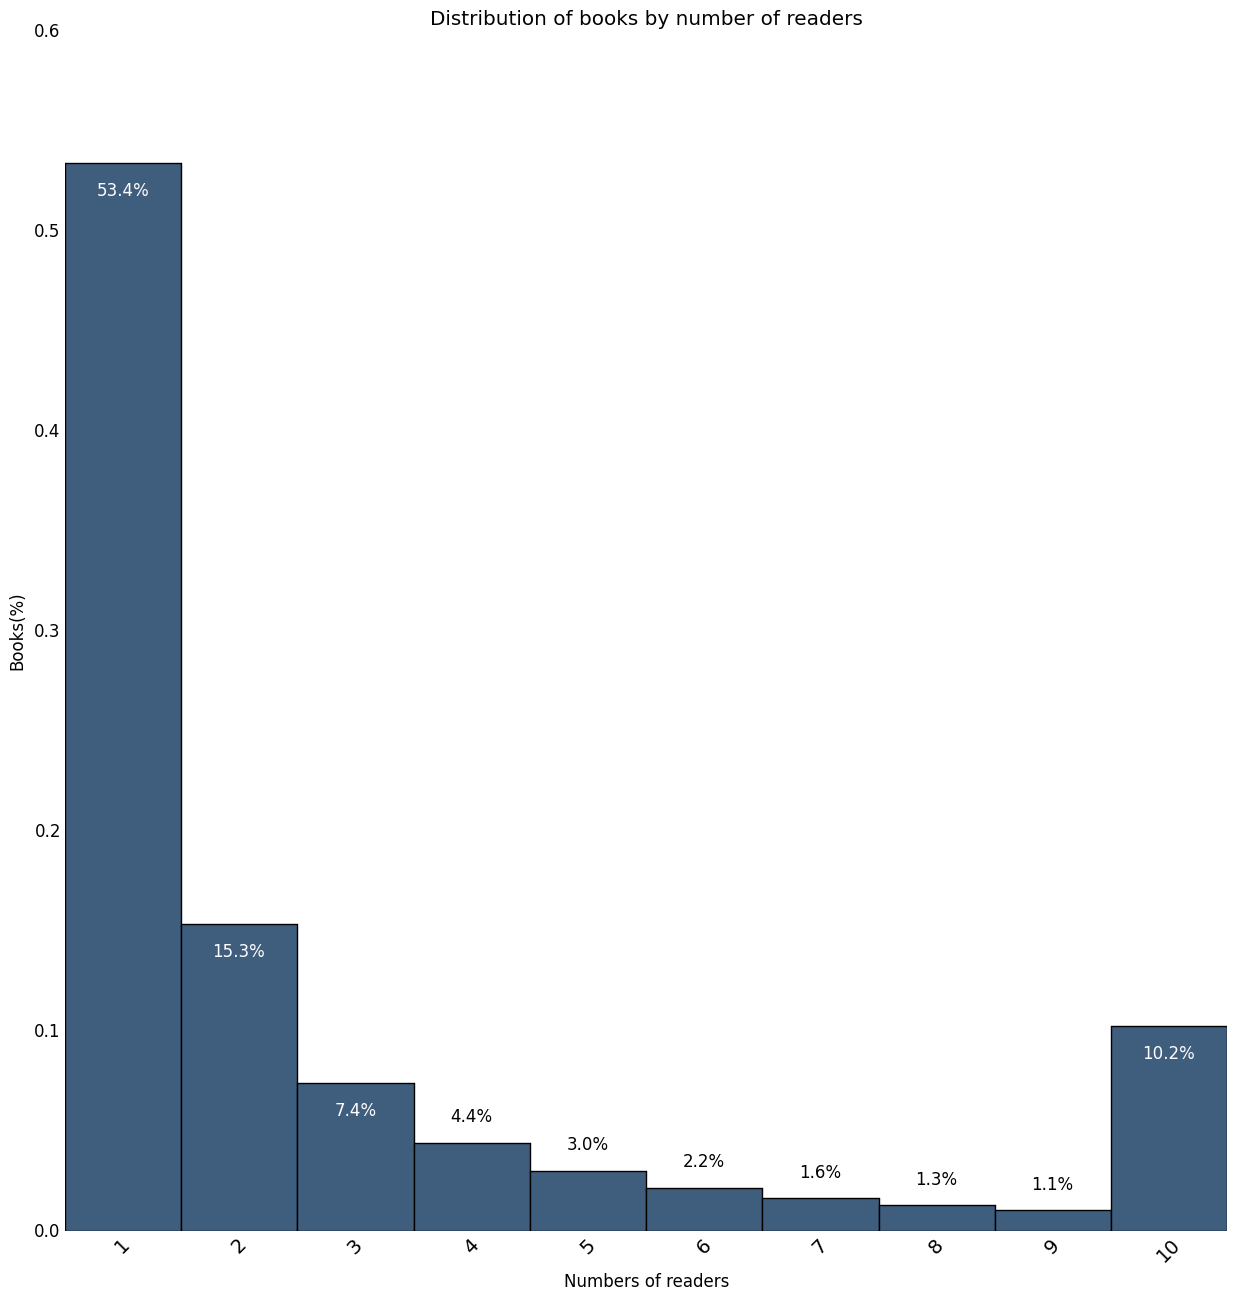
\includegraphics[width=\textwidth]{images/books}
                \caption{Distribution of books}
                \label{fig:books_books_read}
        \end{subfigure}
        \caption{Distribution of books and readers}
\end{figure}

% Books read: 1714613

% !!!!!!always fix bucket size of the column depending on the data!!!!

% User to book
% ------------

% column chart 
% average How many books a user has read - - I want total average



\begin{figure}
        \centering
        \begin{subfigure}[b]{0.5\textwidth}
                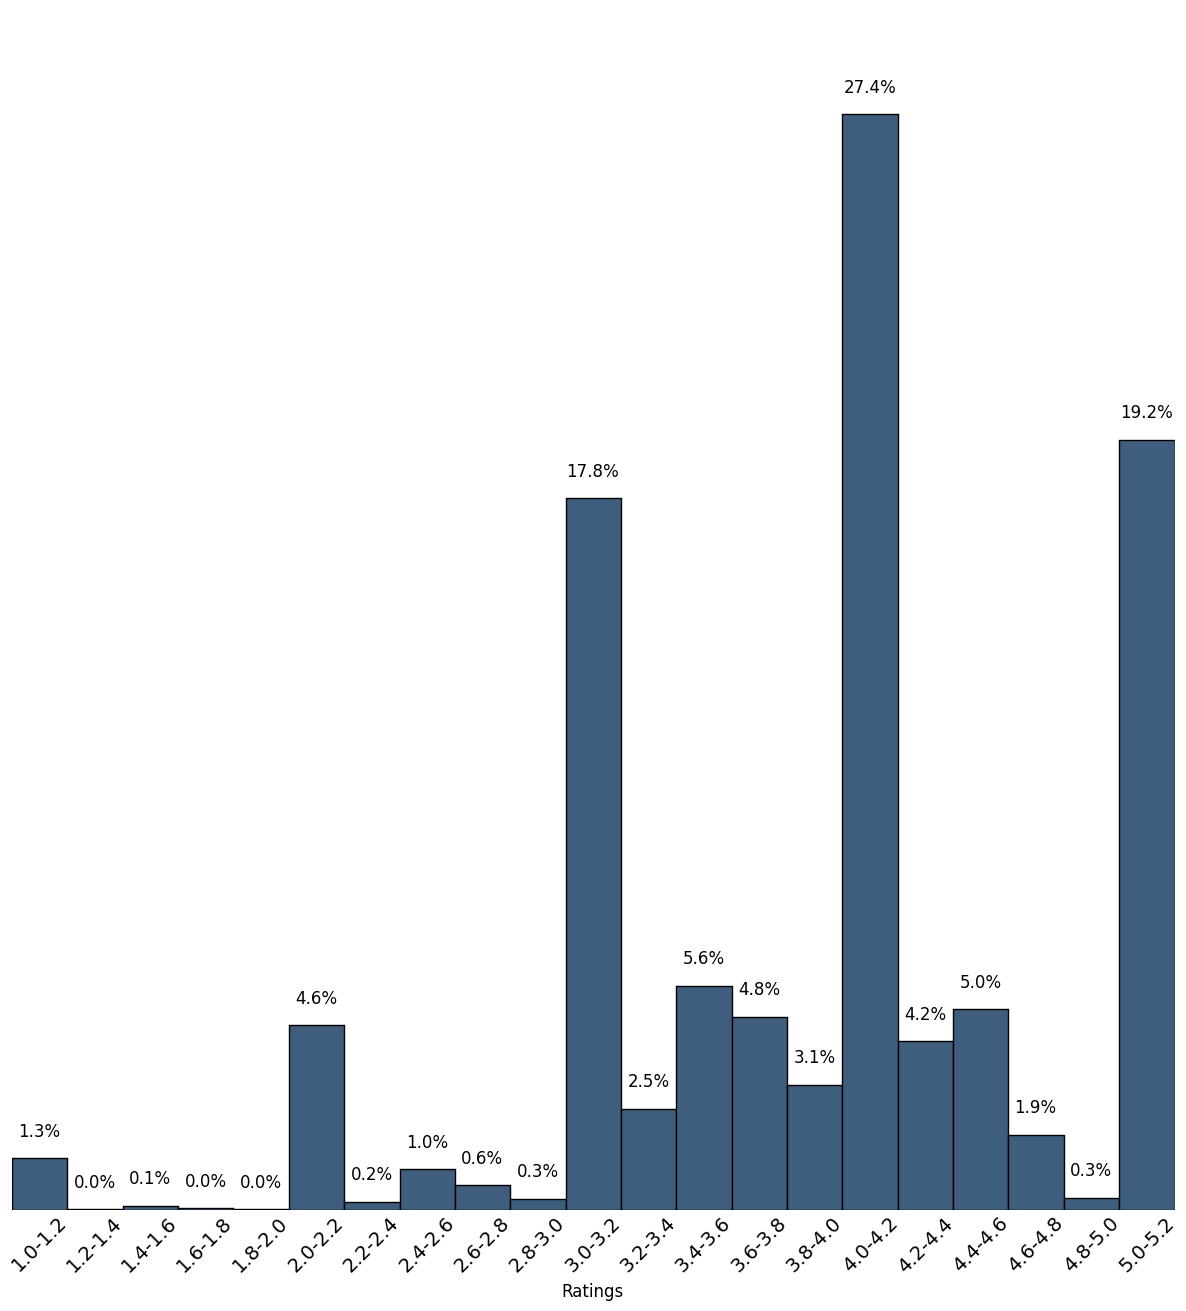
\includegraphics[width=\textwidth]{images/books_ratings}
                \caption{Distribution of books average ratings}
        \end{subfigure}%
        ~ %add desired spacing between images, e. g. ~, \quad, \qquad, \hfill etc.
          %(or a blank line to force the subfigure onto a new line)
        \begin{subfigure}[b]{0.5\textwidth}
                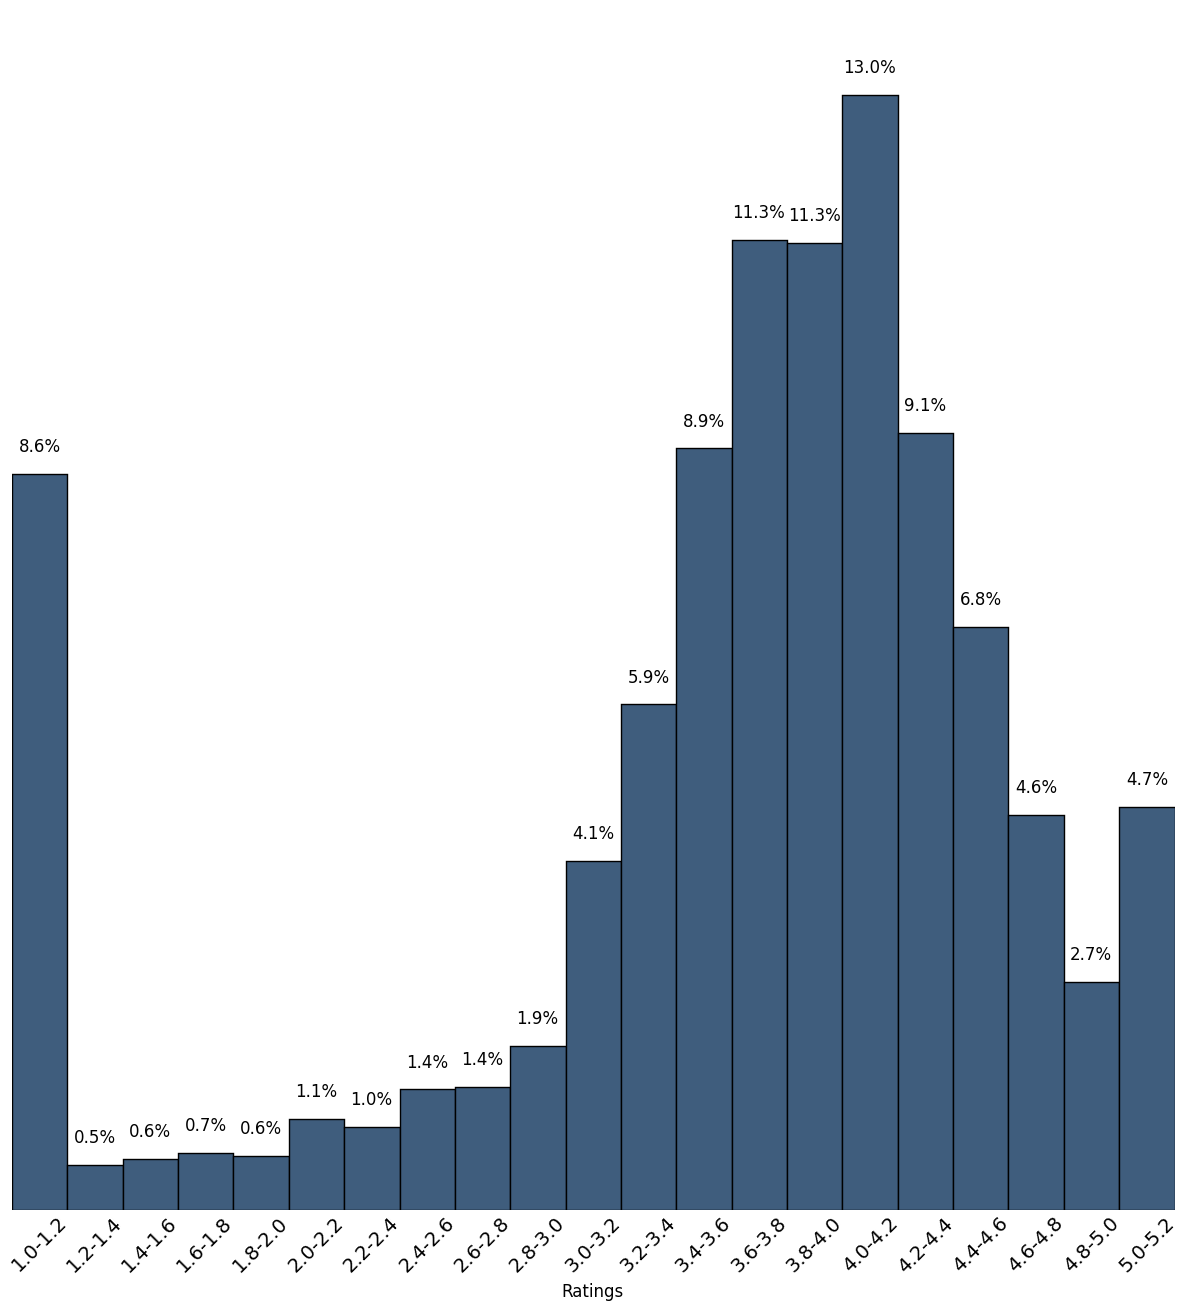
\includegraphics[width=\textwidth]{images/user_ratings}
                \caption{Distribution of readers average rating}
        \end{subfigure}

        \begin{subfigure}[b]{0.5\textwidth}
                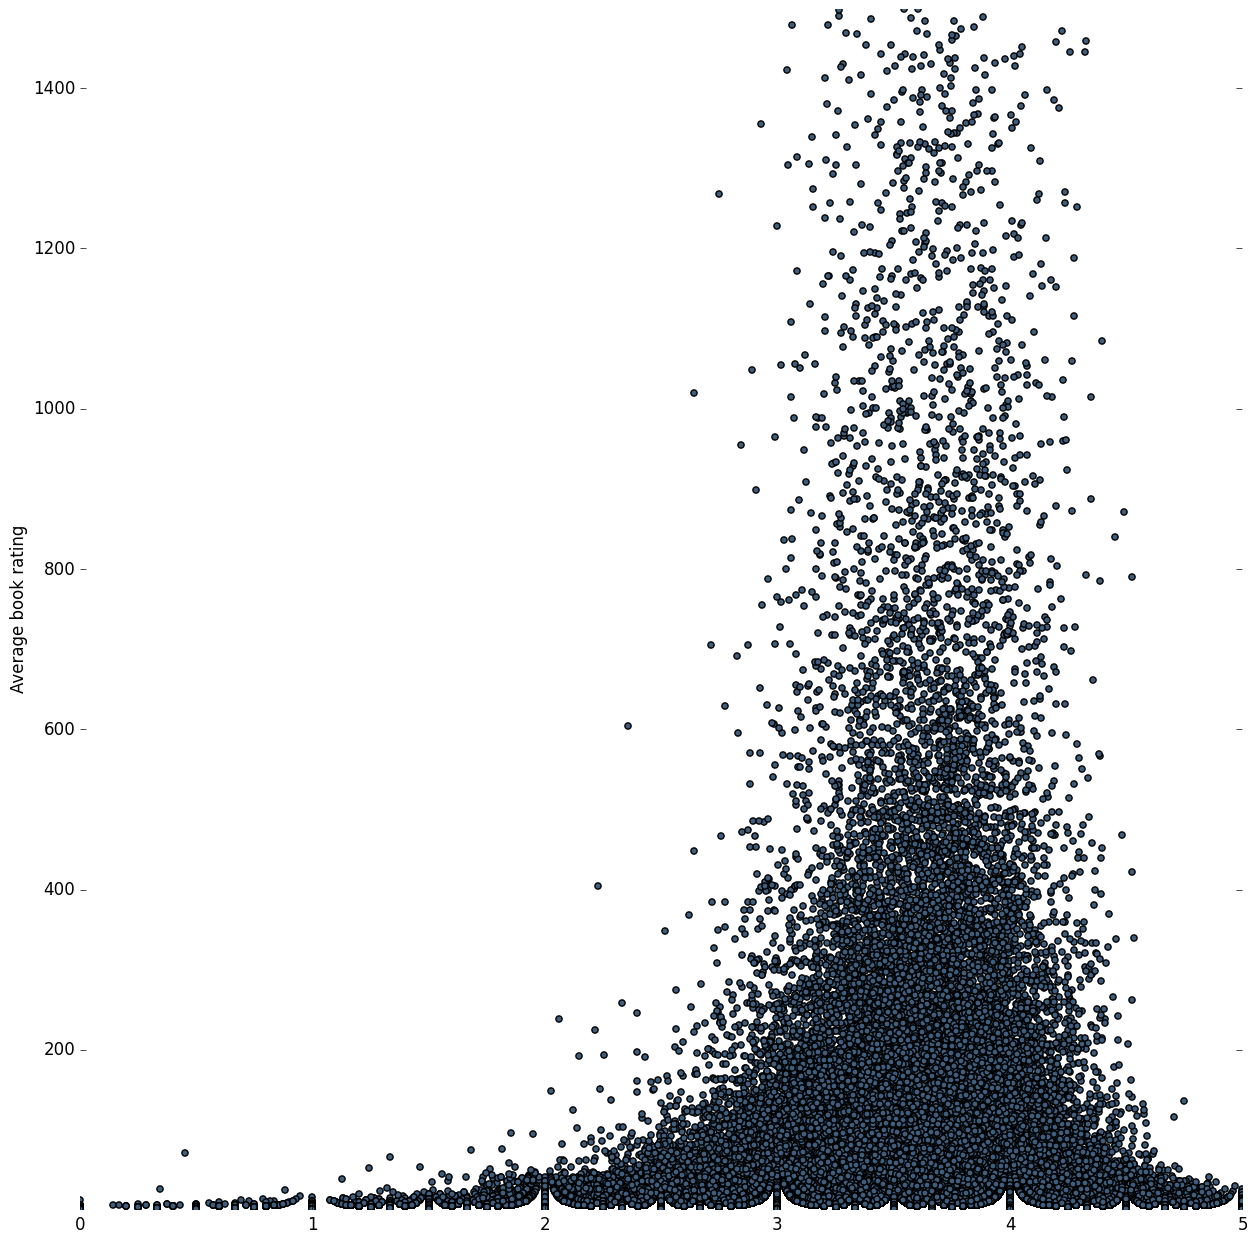
\includegraphics[width=\textwidth]{images/book_scatter_1500}
                \caption{Books per average rating}
        \end{subfigure}%
        ~ %add desired spacing between images, e. g. ~, \quad, \qquad, \hfill etc.
      %(or a blank line to force the subfigure onto a new line)
        \begin{subfigure}[b]{0.5\textwidth}
                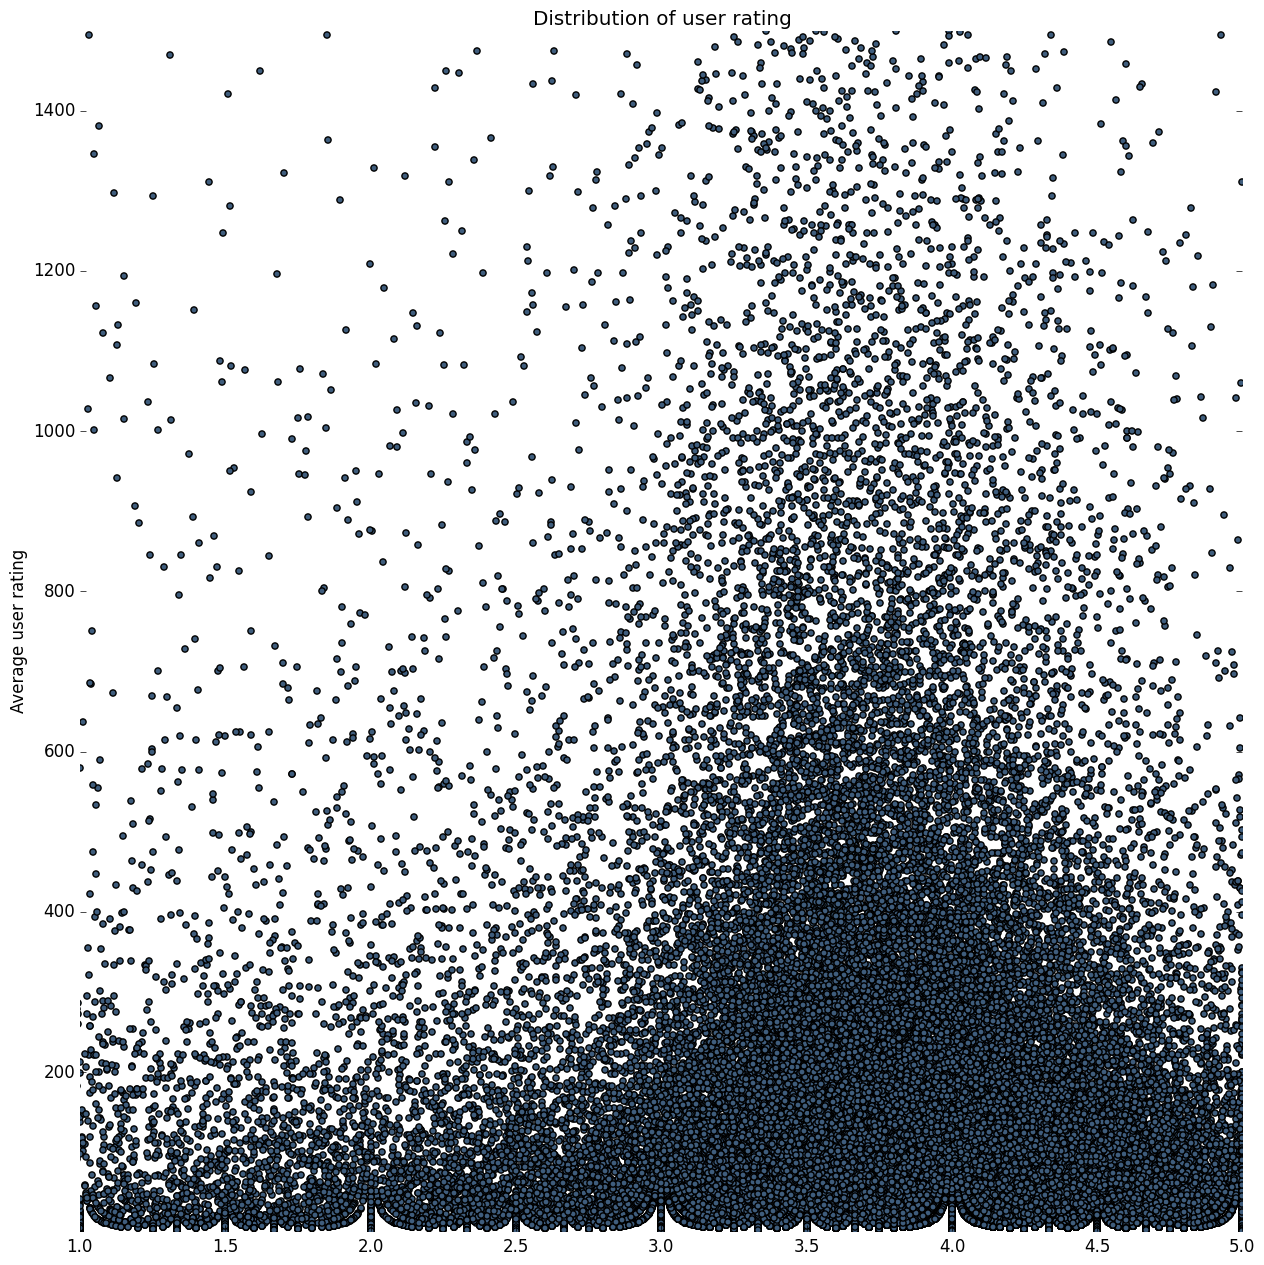
\includegraphics[width=\textwidth]{images/user_scatter_1500}
                \caption{Readers per average rating}
        \end{subfigure}
        \caption{Distribution of ratings for readers and books}
        \label{fig:scatters}
\end{figure}

About the distribtion of ratings, both books and readers have a similar distribution as seen in Figure~\ref{fig:scatters}. However, we notice that the readers ratings are more spread than the books\' ones.


\section{Description of the method}
\label{sec:method}
% Right about score functions - sab kuch
\subsection{Score Function}
As stated earlier, the objective of the current study is to explore the homophily in the goodreads network.
Homophily, the concept in the Social Network Analysis, tries to reason the existence of ties among different vertices in the network.
Homophily says that ties exist between vertices which share similar properties.
These properties depend on the type of social network under the study.
For instance, in a citation network, research domains characterize authors whereas in an online dating network users\' hobbies, mutual interests are the driving force for initiating ties among the users. Goodreads network not only has reading groups of users but also has the provision to become a friend of user.
In this study, we want to reason the ties which goodreads have as a part of friendship graph.\\\\
One can think about many reasons which leads a user to connect to another user on goodreads.
We need to quantify this notion so as to make observations.
We use different score functions while generating a user-user graph from the scraped data.
For each pair user-user, a score function quantifies a kind of homophily which we want to study.
We have considered following score functions.

\begin{description}
	\item[Common Books] Given two users, the homophily is defined by the number of books both users have read in common.
    \item[Common Books Normalized] Given two users, the homophily is defined by the number of books both users have read in common, normalized by the number of books both users have read in total.
    \item[Rating Based] It builds on the earlier score by incorporating the rating given by the users to the books they have read. Given two users, we compute the number of {\it similar}\footnote{For instance, ratings differ by one} ratings, normalized by the number of common books both uesrs have read.
    \item[High Rating Based] This score behaves the same as \textit{Rating Based} except we give a higher weight to high scores.
    If both users have given a 5 rating to the same book, the score will be highers than if they have both rated it 2. 
\end{description}


First and second score function show how similar books user have read whereas others are more subtle looking at whether the users have liked the books they have read. The fourth score is based on the fact that a reader is more defined by the books he likes than the books he does not like. We construct user-user graphs using these score functions and scraped data.

\subsection{Sampling}
We want to find the communities in the user-user graph formed in this way. Nonetheless, the number of users is prohibitive to obtain the communities in the network in considerable amount of time. A few techniques can be employed to reduce the number of users:
\begin{description}
	\item[Reviews Sampling] Instead of considering all reviews, we can consider only a fraction of them. However, random sampling fails to capture important users since this technique may not consider all the books which a user has read. We did \textbf{not} use it.
    \item[Users Sampling] In this technique, we directly sample desired number of users from a set of users. Then we use all the books read by the sampled set of users to create user-user matrix. This sampling method is fair.
    \item[Active Users] It can be clearly observed that, there is a large fraction of users who have read very few books. It may be advantageous to focus the study on voracious readers. These are the readers who have read many books and reviewed them. We can choose the users who have read at least $k$ books. One can tune $k$, to get desired number of users.
    \item[Edges Filtering] Even after sampling the readers, a 10000 readers sample can generate 25 million edges if the user-user graph density is still 50\%. Given that each edge has a score, we can filter them and take the $n$ highest edges.

\end{description}
We have implemented {\it users sampling}, {\it active users} and {\it edges filtering}.

\subsection{Community Detection}
Once the communities are found we proceed to calculate homophily in the network. To calculate the homophily, we use the friendship information related to users. Let $S$ denote the set of users in a graph and $f(u)$ denotes set of friends of user $u$($\in S$) in $D$. Let $\mathcal{C}$ be the set of communities returned by community detection algorithm. Homophily of cluster $C_i$ is calculated as:
\[
\mathcal{H}_{C_i} = \sum_{v \in C_i} \frac{|C_i \cap f(v)|}{|f(v)|}
\]
We use the homophily of the cluster to find global homophily for the graph. It is weighted sum of cluster homophily. It is given by:
\[
\mathcal{H}_{S} = \sum_{C_i \in \mathcal{C}} w_{C_i} \mathcal{H}_{C_i} ~~~~~~~~~\textrm{where,}~~~w_{C_i} = \frac{|C_i|}{|S|}
\]
Since the homophily calculation relies heavily on the community detection algorithm, use of a single community detection algorithm may make the analysis biased. So as not to make the analysis partisan we use two different algorithms for analyzing user-user graph.\\\\
In this way, {\it Score Function}, {\it Sampling} and {\it Community Detection} are the dimensions along which we analyze the homophily in goodreads community.

\section{Challenges}
We encountered many challenges at different stages of the project. Here we enlist them one by one.

\subsection{Data processing}
Each information needs a request to goodreads to fetch the data. To gather data related to a user, namely friends and books, a lot of queries have to be fired to goodreads. For close to $86000$ users, we made more than 1 million requests. We used multiprocessing to expedite this process.

\subsection{Matrix projection}
We need to generate user-user matrix from a bipartite network comprising of approximately $86000$ users, $1.7$ million books and $14$ million edge. Although the bipartite network is sparse, the resultant one mode projection is highly dense. When we got memory issues with {\it networkX} we used {\it scipy} as a resort. But even with scipy, the projected matrix being very dense, memory issues persisted\footnote{ We hit a memory overflow on a machine with 64GB of main memory.}. Plus the community detection algorithms have very poor running time for large graphs. To skip both of these hurdles, we used sampling techniques as described in Section \ref{sec:method}

\subsection{User-User Graph}
Use of matrix multiplication is a classical way to compute one mode projection. But the objective of the study is directed more towards semantics of the ties, we compute each edges between two users by hand making use of score functions defined in Section \ref{sec:method}. As we need to compute the edge weight between every pair of two readers, to build a graph with $n$ users, we must iterate over $n \choose 2$ edges. For 10000 users, we have to compute 50 million edges. Again we use multiprocessing, to expedite this user-user graph generation.

%\textbf{Success Measure}\\
%Homophily talks about the existence of strong ties within the nodes in a social network. Naturally, people sharing similar interests tend to get connected with each other leading to the formation of the strong ties amongst them. In this project, we explore the extent to which the groups on goodreads adhere to homophily.\\\\
%We propose to explore this by studying the one-mode projection on the users. Affiliation network, a bipartite network between users and books, is used to calculate the projection on the users and hence, users having read some common books are associated in the user matrix. We further find the communities in this network to study homophily. If the users in a community are indeed friends on goodreads, then it explains that there is no external bias in the friendship observed in goodreads social network.\\\\
%To quantify it for a certain community, consider $\mathcal{U}(V_u, E_u)$, projected user matrix and $\mathcal{F}(V_u, E_f)$ friendship network in goodreads. Let $\mathcal{C}(V_c, E_c)$ be a community in $\mathcal{U}$. The extent of homophily in community $\mathcal{C}$ is given by $\frac{|E_c \cap E_f|}{|E_c|}$.

\section{Evaluation}


\begin{table}[ht]
\begin{center}
\begin{tabular}{lcccc}
\hline
Size Sample (thousand) & Sampling Users  &   Score function &  Size Edges (million) &  Detection Algorithm & Number of clusters & Global homophily \\ \hline
3  & Random         & Common             &  1.9  &  louvain  & 4 &  0.133
3  & Random         & Common             &  1.9  &  walktrap  & 153 &  0.007
3  & Random         & High Rating             &  1.8  &  louvain  & 4 &  0.12
3  & Random         & High Rating             &  1.8  &  walktrap  & 153 &  0.007

\end{tabular}
\end{center}
\caption{Goodreads Authors/Users Statistics}
\label{table:crawl_stat}
\end{table}


\section{Outline of each team member's contributions}


\bibliographystyle{abbrv}
\bibliography{final_ref}
\end{document}
